\documentclass[my_thesis.tex]{subfiles}

\begin{document}
\chapter{Equilibrium beta limits of canonical configurations} \label{ch5.equilibrium_beta_limit}

In magnetic fusion devices such as stellarators, zeroth order confinement of particles and energy is obtained by constructing an equilibrium with magnetic surfaces.
Magnetic islands and magnetic field line chaos can be detrimental to confinement, \textit{i.e.} they can contribute to increased radial transport of particle and energy \citep{Hudson2010}.
While it is possible to design equilibria with good magnetic surfaces in a vacuum \citep{Cary1985,Cary1986,pedersenConfirmationTopologyWendelstein2016}, pressure-driven plasma currents, such as diamagnetic, Pfirsch-Schl\"uter and bootstrap currents, perturb finite pressure equilibria, and, at a sufficiently large pressure, magnetic islands and chaos emerge. 


A pressure increase can also sometimes heal magnetic islands \citep{Bhattacharjee1995}. While this mechanism can improve confinement locally, other islands might open elsewhere in the plasma as $\beta$ increases.
There is thus a critical value of $\beta$ at which magnetic islands open and magnetic field line chaos emerges. This defines an \emph{equilibrium $\beta$-limit}.
Note however that the equilibrium $\beta$-limit is a "soft" limit, since crossing it does not lead to a loss of control of the plasma. Additional input power may however leak through the damaged magnetic surfaces more easily \citep{rechesterElectronHeatTransport1978}, thereby preventing an increase of $\beta$. Crossing the equilibrium $\beta$-limit may thus not be as concerning as crossing a stability limit (which may lead to plasma disruptions), but it still limits the overall performance of the reactor. It is consequently of crucial importance to understand these equilibrium $\beta$-limits better, especially for the operation of existing experiments and the design of new machines. Configurations where good magnetic surfaces are preserved over a large range of $\beta$ have to be sought, which will help to ultimately identify configurations whose equilibrium $\beta$-limit is large enough.


\section{Classical stellarator}


In the case of a classical stellarator, \citet{Loizu2017} proposed a model for the equilibrium $\beta$-limit of a configuration with zero net toroidal current as well as one with a fixed edge rotational transform. 
Other studies computed high $\beta$ equilibria in a number of experimentally relevant stellarator configurations and predicted the emergence of magnetic field line chaos at sufficiently large $\beta$ - see, for example, the calculation by \citet{suzukiTheoreticalStudiesEquilibrium2020} in the Large Helical Device (LHD) and \citet{Reiman2007} in Wendelstein 7-AS (W7-AS). However, to the authors knowledge, no attempt has been made to analytically model the impact of the bootstrap current on the equilibrium $\beta$-limit, and to determine how this critical $\beta$ depends on the device parameters.

%We use the Stepped Pressure Equilibrium Code (SPEC) to compute a large number of free-boundary equilibria at different $\beta$, including the effect of bootstrap current. SPEC has been chosen for its speed, its capability to describe equilibria with magnetic islands and chaos, and the possibility to calculate free-boundary equilibria \citep{Hudson2020c} with a constrained toroidal current profile \citep{Baillod2021}. SPEC has been verified in stellarator geometry \citep{Loizu2016}, and its core algorithm has been improved to run faster and to be more robust \citep{Qu2020}. It has been successfully applied to study current sheets at rational surfaces \citep{Loizu2015,Loizu2015a,huangNumericalStudyFunction2022}, ideal linear instabilities \citep{Kumar2021,Kumar2022}, tearing mode stability \citep{Loizu2019} and non linear saturation \citep{Loizu2020}, penetration of resonant magnetic perturbations in the ideal limit \citep{Loizu2016a} and relaxation phenomena in reversed field pinches \citep{Dennis2013a,Dennis2014,quSteppedPressureEquilibrium2020}.

%To numerically identify the equilibrium $\beta$-limit, \citeauthor{Loizu2017} used a diagnostic based on the \emph{volume of chaos}, \textit{i.e.} the volume of plasma occupied by chaotic field lines, which were identified by measuring their fractal dimension \citep{Meiss1992c}. However, this approach is too pessimistic since some chaotic magnetic field lines might be able to preserve confinement \citep{Hudson2008}. An alternative approach, proposed by \citet{paulHeatConductionIrregular2022}, is to measure the \emph{effective volume of parallel diffusion}. This measures the fraction of plasma volume over which the local parallel transport dominates over the perpendicular one in setting the radial transport. Contrary to the volume of chaos,  this approach takes into account only sufficiently large resonances that do participate significantly to the radial transport. In this paper, we follow \citeauthor{paulHeatConductionIrregular2022} and measure the \emph{equilibrium $\beta$-limit} by taking the $\beta$ above which the radial transport generated by damaged magnetic surfaces represents a significant fraction of the total radial transport.

We propose to extend the work of \citet{Loizu2017} to the case of a classical stellarator with bootstrap current. While a rotating ellipse is arguably a simple geometry, it is still relevant since all stellarators without torsion are rotating ellipses close to the magnetic axis \citep{helanderTheoryPlasmaConfinement2014}. An experimental instance of rotating ellipse was, for example, the Wendelstein VII-A stellarator \citep{Grieger1985}.

We choose a computational boundary $\Gamma_{CB}$  (see Figure \ref{fig. modB boundary}) using standard cylindrical coordinates $\mathbf{x}=R_{CB}(\theta,\phi)\mathbf{\hat{e}}_R +Z_{CB}(\theta,\phi)\mathbf{\hat{e}}_Z$, with
\begin{align}
	R_{CB}(\theta,\phi) &= R_0 + R_{10}\cos(\theta) + R_{11}\cos(\theta-N_{fp}\phi)\label{eq.cb_r}\\
	Z_{CB}(\theta,\phi) &= Z_{10}\sin(\theta) + Z_{11}\sin(\theta-N_{fp}\phi)\label{eq.cb_z},
\end{align}
with $N_{fp}=5$ the number of field periods, $R_0=10$m, $R_{10}=-Z_{10}=1$m, $R_{11}=Z_{11}=0.25$m. The effective minor radius is $a_{\text{eff}}=\sqrt{r_{min}r_{max}}$ with $r_{min}=R_{10}-R_{11}$ and $r_{max}=R_{10}+R_{11}$ the minor and major radii of the ellipse respectively. We define $\epsilon_a=a_{\text{eff}}/R_0$ as the inverse aspect ratio.


\begin{figure}
	\centering
	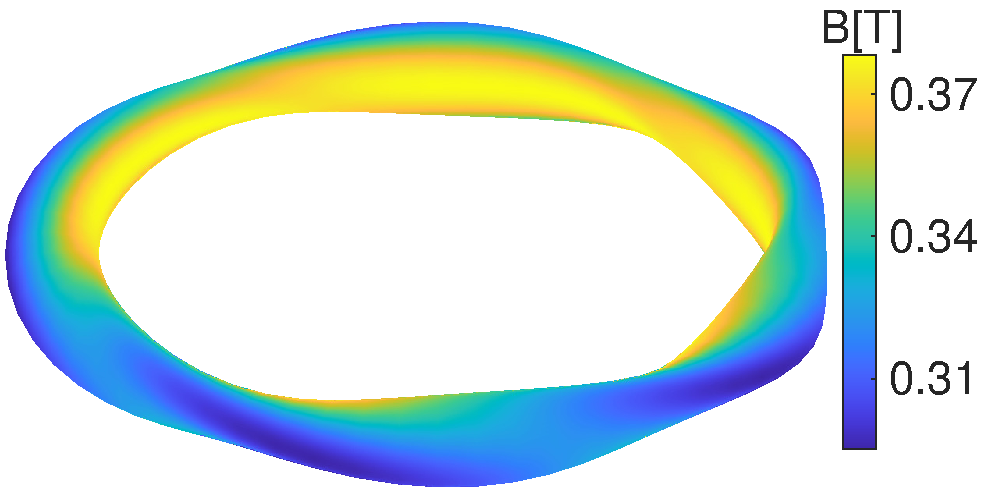
\includegraphics[width=.7\linewidth]{images/ClassicalStellaratorBetaLimit/ComputationalBoundary_modB.pdf}
	\caption{Computational boundary described by Eqs.(\ref{eq.cb_r})-(\ref{eq.cb_z}). Colors indicate the magnetic field strength in vacuum.}
	\label{fig. modB boundary}
\end{figure}

We assume that a coil system exists such that $\mathbf{B}_c\cdot\mathbf{n}=0$ on $\Gamma_{CB}$, where $\mathbf{B}_c$ is the magnetic field produced by the coils, and we fix the total coil current to $I_c=17.1$MA.
Also, an additional external vertical field, $\mathbf{B}_v=B_v\mathbf{\hat{e}}_Z$ is applied to keep the plasma within the computational boundary at high-$\beta$. We set $B_v=-0.03$T. This vertical field has little to no impact on the results presented hereafter; its only purpose is to keep the plasma within the volume defined by $\Gamma_{CB}$. 


We choose a pressure profile with a linear dependence on the toroidal flux, \textit{i.e.} $p=p_0(1-\psi_t/\psi_a)$, with $p_0$ a free parameter and $\psi_a=0.25\text{Tm}^2$ the total toroidal flux enclosed by the plasma boundary $\Gamma_{PB}$. We approximate the pressure profile with seven steps of equal magnitude $[[p]]_l=p_0/N_{vol}$. We thus define seven plasma regions, \textit{i.e.} $N_{vol}=7$, surrounded by a vacuum region. This means that $\psi_{t,l}=(l-1)\psi_a / N_{vol}$ and $p_l=p(\psi_{t,l})$. The number of volumes determines how the pressure profile is represented --- more volumes means more and smaller pressure steps. As each interface is a discrete constraint on the magnetic topology, increasing the number of volumes reduces the available space for reconnection and thus the maximum size of magnetic islands and regions of magnetic field line chaos.  In this paper, we are however interested in the onset of loss of magnetic surfaces, which is not affected by the volume available for islands to grow. Therefore our results are very weakly dependent on the number of volumes.

%The question remains: what is the adequate number of volumes to represent the actual, real-world physics? {\color{red} This is unclear. Need to figure out good argument. The stochastization begins in vacuum argument does not work, since we changed the diagnostic... I am now running a case with two volumes for comparison.}

%Observations showed however that this phenomenon occurs first in the vacuum region, on the outer side of $\Gamma_{PB}$, where the magnetic topology is unconstrained no matter the number of volumes and then propagate in the plasma region if $\beta$ is increased. In this paper, we focus on the critical $\beta$ at which
%The number of plasma volumes defines with how many steps the pressure profile is approximated with --- increasing the number of volumes thus increases the resolution of the pressure profile. 
%As each volumes' interface is constrained to be a magnetic surface, increasing the number of volumes reduces the volume in which reconnection can occur. In other words, increasing the number of volumes increases the number of topological constraints. In fact, \citet{Dennis2013} proved that in the limit of infinite number of volumes, ideal MHD is retrieved.


%In experiments, magnetic field line chaos first emerges at the plasma edge and then moves towards the center \citep{Reiman2021}; this is also observed in our results. Since chaotic regions appear first outside the plasma boundary, which is free from any constraint on the magnetic topology (there are no interfaces between $\Gamma_{PB}$ and $\Gamma_{CB}$), the critical $\beta$ at which stochastization occurs is unaffected by the number of volumes. This paper will focus on this critical $\beta$; what happens after the onset of stochastization is not important here, and thus the results presented in this paper are independent of the number of volumes.

Finally, two current profiles have to be provided to SPEC: the profile of volume currents, $\{I^v_{\phi,l}\}$, and the profile of surface currents $\{I^s_{\phi,l}\}$ (see section \ref{sec. current constraint}). Here we study the case of an equilibrium with zero externally driven currents and with bootstrap current. No externally driven currents implies, in SPEC, that there are no currents in the plasma volumes, \textit{i.e.}
\begin{equation}
	I^v_{\phi,l} = 0.\label{eq.volume current}
\end{equation}
	
The bootstrap current is a pressure-driven current, and is consequently described by a surface current at the volume's interfaces. We model it with
\begin{equation}
	I^s_{\phi,l} = -C \left(\frac{\psi_{t,l}}{\psi_a}\right)^{1/4} \left[\left[p\right]\right]_l, \label{eq.bootstrapmodel}
\end{equation}
where $(\psi_t / \psi_a)^{1/4}\approx\sqrt{\epsilon}$ is related to the fraction of trapped particles, with $\epsilon$ the inverse aspect ratio; $[[p]]_l$ is a measure of the local pressure gradient; and $C$ is a coupling constant, in $[APa^{-1}]$, which controls the strength of the bootstrap current in the system. 
A full neoclassical calculation of the bootstrap current, for example with the SFINCS code \citep{landremanComparisonParticleTrajectories2014}, would require the density and temperature profiles as inputs --- and the freedom in the choice of the coupling constant $C$ reflects the freedom in these profiles. 

	

The current density associated to the current in Eq.(\ref{eq.bootstrapmodel}) is
\begin{equation}
	j_{\phi,l} = -\frac{C\psi_a}{\pi a_{\text{eff}}^2}\left(\frac{\psi_{t,l}}{\psi_a}\right)^{1/4}\frac{dp}{d\psi_t}. \label{eq.current density continuous}
\end{equation}	
Note that if 
\begin{equation}
	C = C_0 \equiv \frac{\sqrt{\epsilon_a}R_0}{\iotabar_v B_0}, \label{eq. def C0}
\end{equation}
with $\iotabar_v$ the edge rotational transform in vacuum and $B_0$ such that $\mu_0I_c= 2\pi R_0 B_0$, Eq.(\ref{eq.current density continuous}) reduces to the well-known large-aspect ratio tokamak bootstrap current approximation \citep{helanderCollisionalTransportMagnetized2002},
	
\begin{equation}
	j_{\phi} = \sqrt{\epsilon_a}R_0\frac{d p}{d\psi_p},
\end{equation}
where $\psi_p$ is the poloidal flux, and we made the approximation $d\psi_p/d\psi_t=\iotabar\approx\iotabar_v$. The constant $C_0$ will be used to normalize $C$, \textit{i.e.} we define $\hat{C}\equiv C / C_0$. In the case of a large aspect ratio circular tokamak, we thus have $\hat C = 1$, while in a stellarator with no bootstrap current, $\hat C=0$.
	
We use the recently implemented capability of SPEC to prescribe the toroidal current profile \citep{Baillod2021}, with the profiles defined in Eqs.(\ref{eq.volume current}) and (\ref{eq.bootstrapmodel}).
Unless stated otherwise, the Fourier resolution used in all results presented in this paper is $|n|\leq N=8$, $m\leq M=8$, with $n$ the toroidal mode number and $m$ the poloidal mode number, meaning that $2[N+M(2N+1)]+1=289$ Fourier modes are used to describe each interface geometry. Results presented in this paper have been checked for convergence with respect to Fourier resolution. 


In summary, we can construct free-boundary SPEC equilibria with a simple bootstrap current model and we are left with two free parameters, namely (i) $\beta$ which controls the total pressure in the system and (ii) $\hat{C}$, a dimensionless parameter, that controls the bootstrap current strength for a given plasma $\beta$. 
	
	
	






\subsection{Scans over $\hat{C}$ and $\beta$}
A scan has been performed with $\beta\in[0,2\%]$ and $\hat{C}\in[0,2.26]$ representing $680$ SPEC calculations, each requiring about $24$ CPU-hours on the MARCONI cluster\footnote{https://www.hpc.cineca.it/hardware/marconi}. Figure \ref{fig. poincare} shows some selected Poincar\'e sections at different values of $\beta$ and $\hat{C}$, while Figure \ref{fig. iota edge} shows the edge rotational transform, \textit{i.e.} the rotational transform on the outer side of $\Gamma_{PB}$, as a function of $\beta$ for four different values of $\hat{C}$.
%Different behavior are observed depending on the value of $\hat{C}$. A critical value of $\hat{C}$, thereafter referred to as $\hat{C}_{crit}=0.59$, determines how the magnetic surfaces are destroyed as $\beta$ increases.

\begin{figure}
	\centering
	\begin{tikzpicture}
		\node[] (p11) at (-3,2) {
			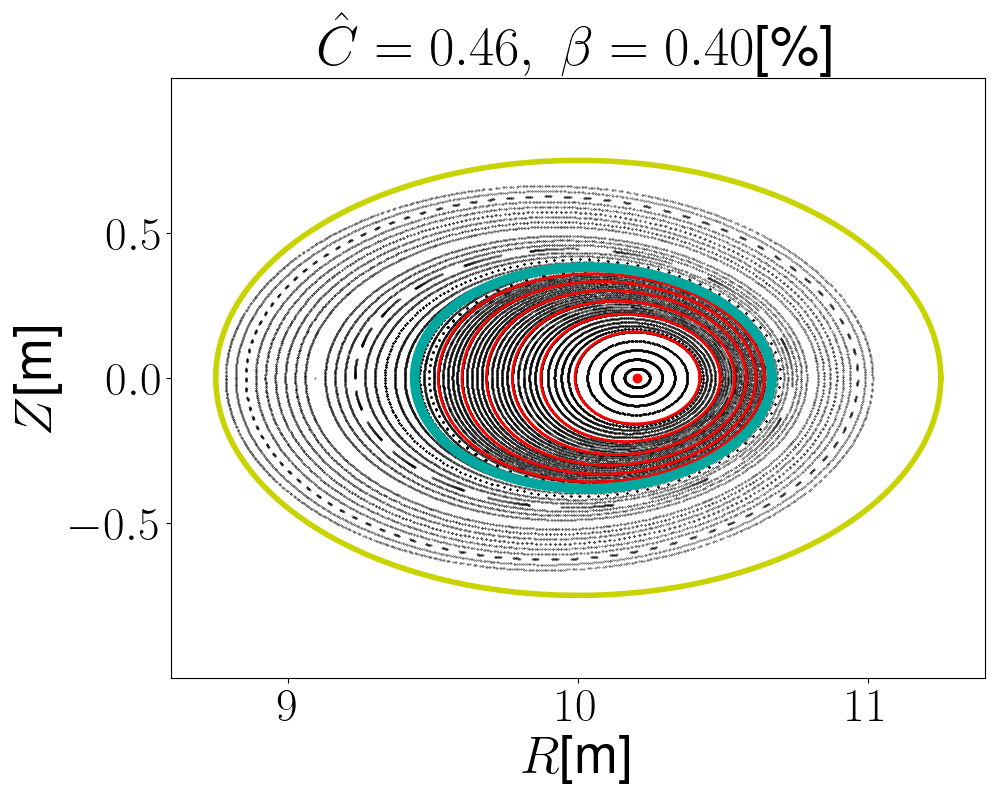
\includegraphics[width=.42\linewidth]{images/ClassicalStellaratorBetaLimit/Poincare_C10_N10.png}	
		};
		\node (p21) at (-3,-2.6) {
			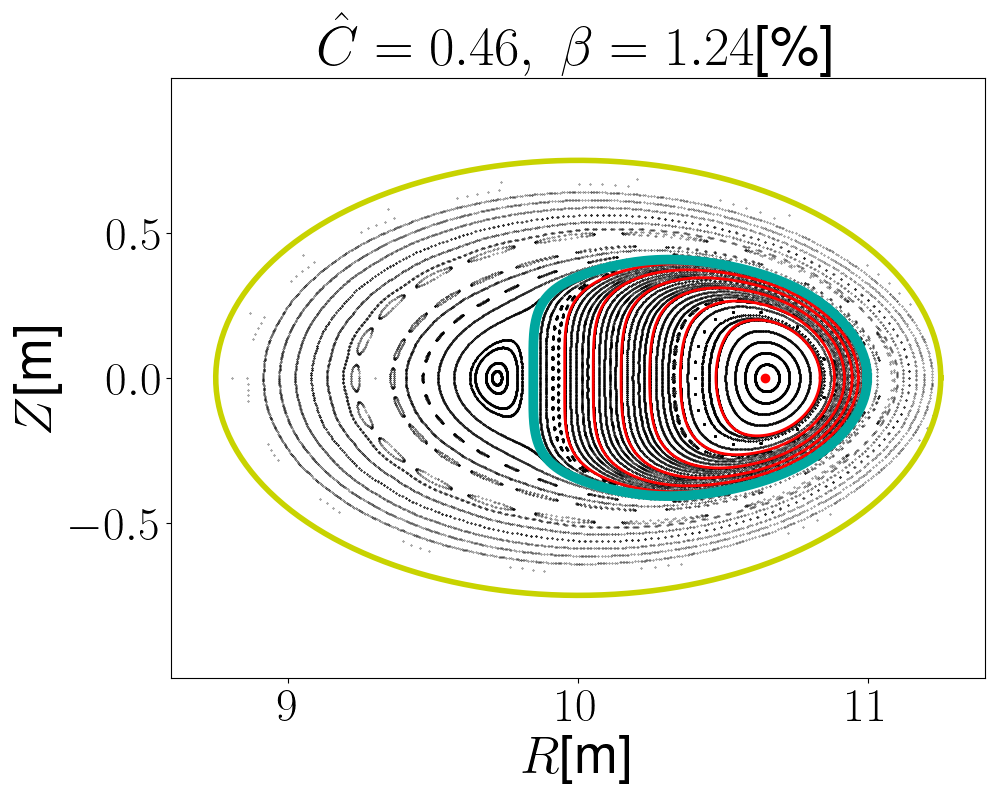
\includegraphics[width=.42\linewidth]{images/ClassicalStellaratorBetaLimit/Poincare_C10_N25.png}	
		};
		\node[] (p11) at (-3,-7.2) {
			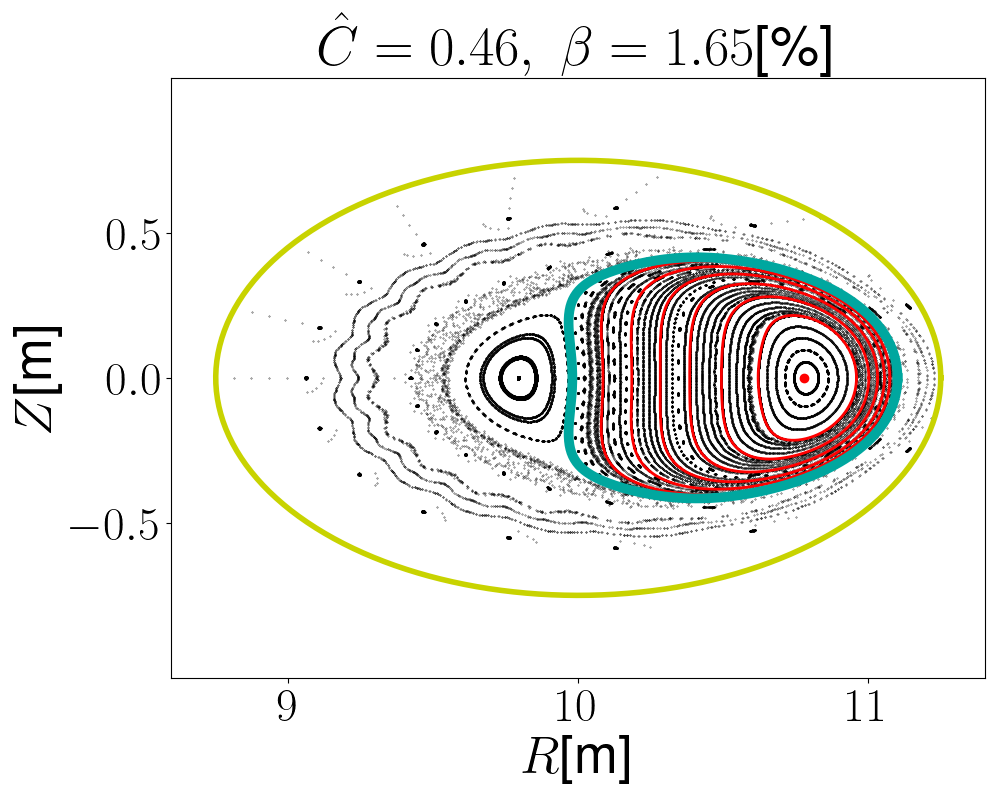
\includegraphics[width=.42\linewidth]{images/ClassicalStellaratorBetaLimit/Poincare_C10_N33.png}	
		};
		\node (p12) at (3,2) {
			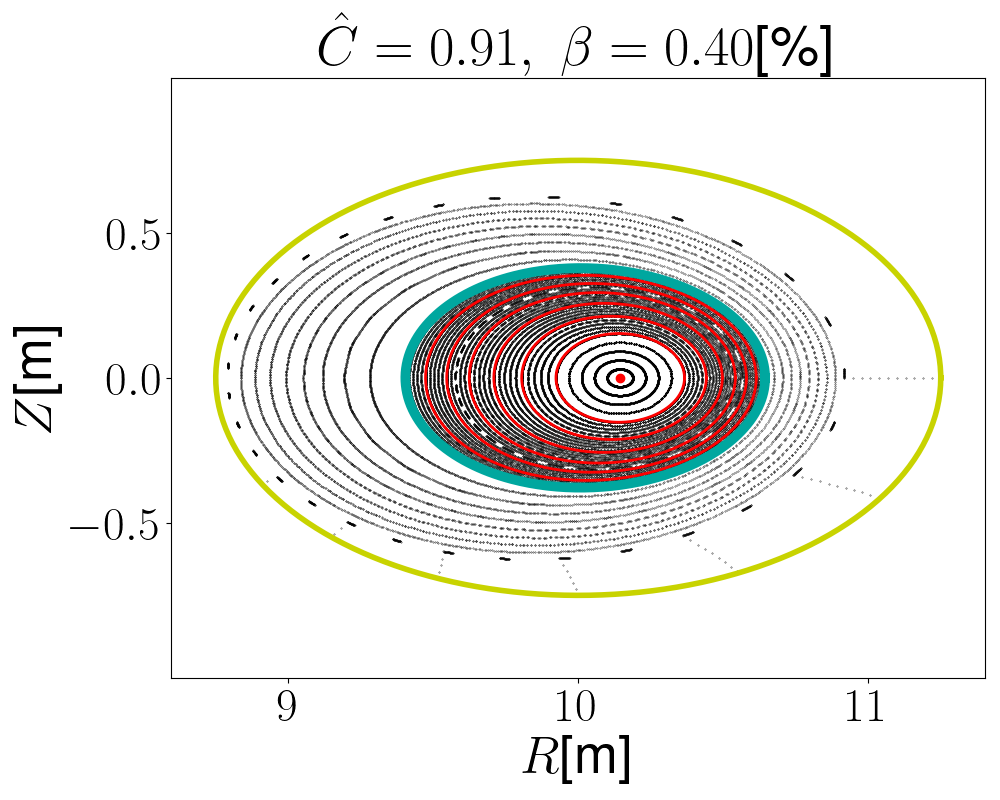
\includegraphics[width=.42\linewidth]{images/ClassicalStellaratorBetaLimit/Poincare_C20_N10.png}	
		};
		\node (p22) at (3,-2.6) {
			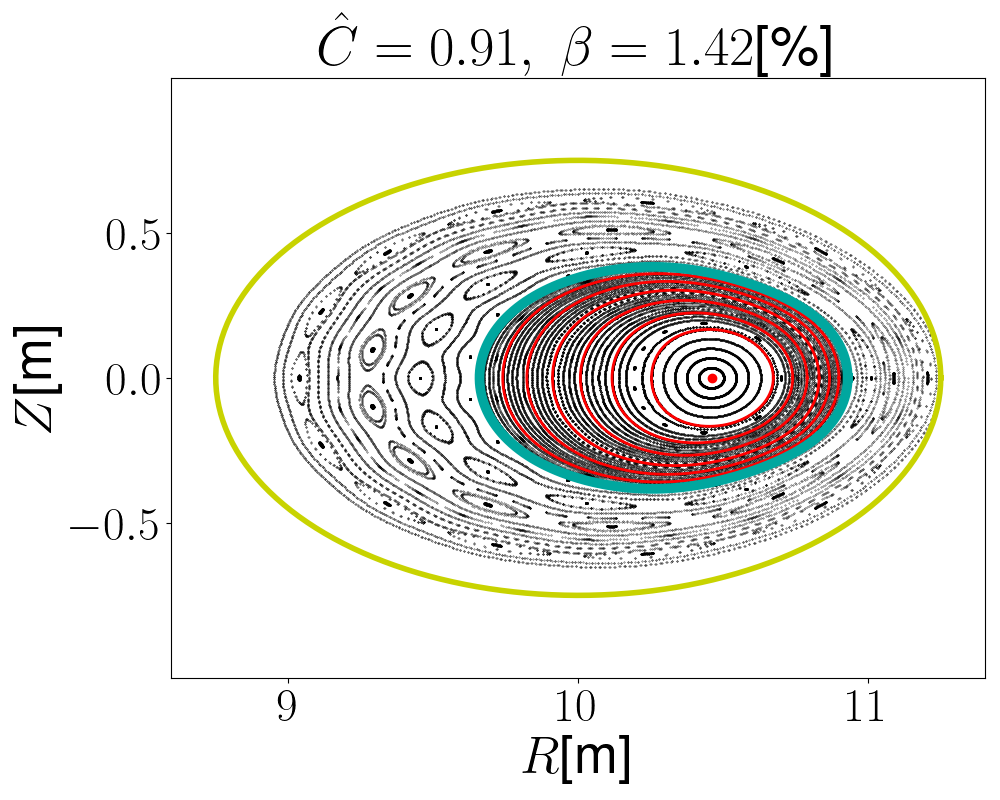
\includegraphics[width=.42\linewidth]{images/ClassicalStellaratorBetaLimit/Poincare_C20_N29.png}	
		};
		\node (p21) at (3,-7.2) {
			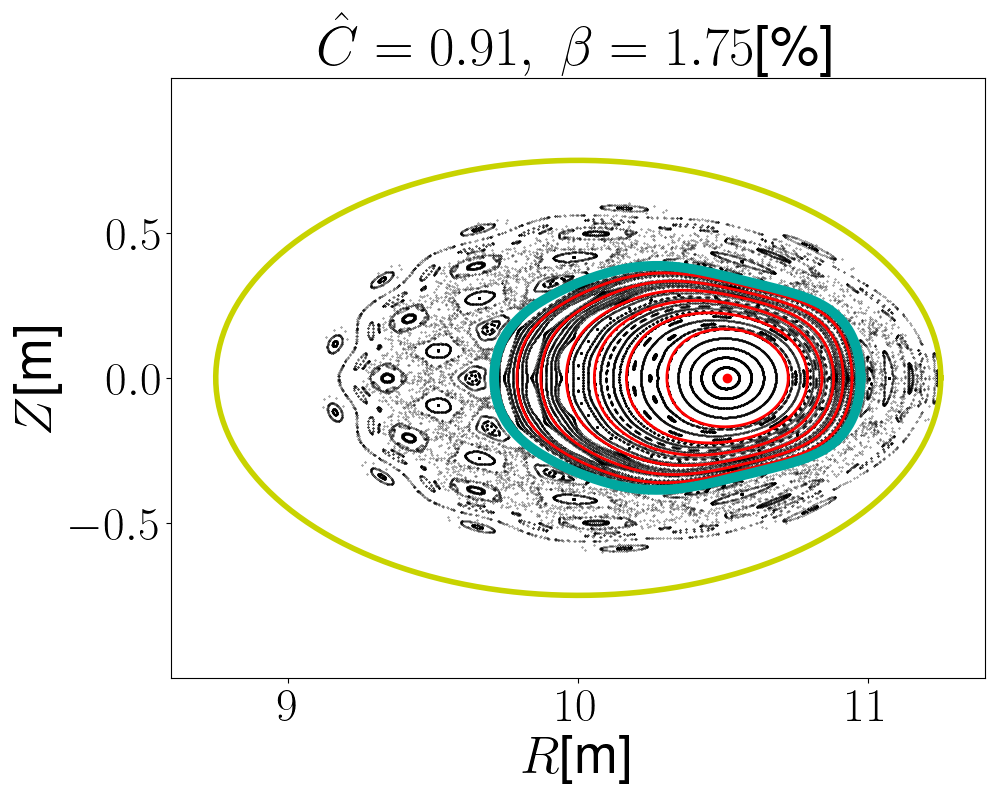
\includegraphics[width=.42\linewidth]{images/ClassicalStellaratorBetaLimit/Poincare_C20_N35.png}	
		};
		\draw[-stealth, very thick] (-6,3)--(-6,-7.7) node [midway, above, rotate=90] {Increasing $\beta$};
		\draw[-stealth, very thick] (-5,4.5)--(5,4.5) node [midway, above] {Increasing $\hat{C}$};	
	\end{tikzpicture}
	\caption{Poincar\'e plot (black dots) of equilibria at toroidal angle $\phi=0$ and at different values of $(\beta,\hat{C})$. Red lines: inner plasma volume interfaces; blue line: plasma boundary; and yellow line: computational boundary.  Left: $\hat{C}=0.46$. Right: $\hat{C}=0.91$.}
	\label{fig. poincare}
\end{figure}



\begin{figure}
	\centering
	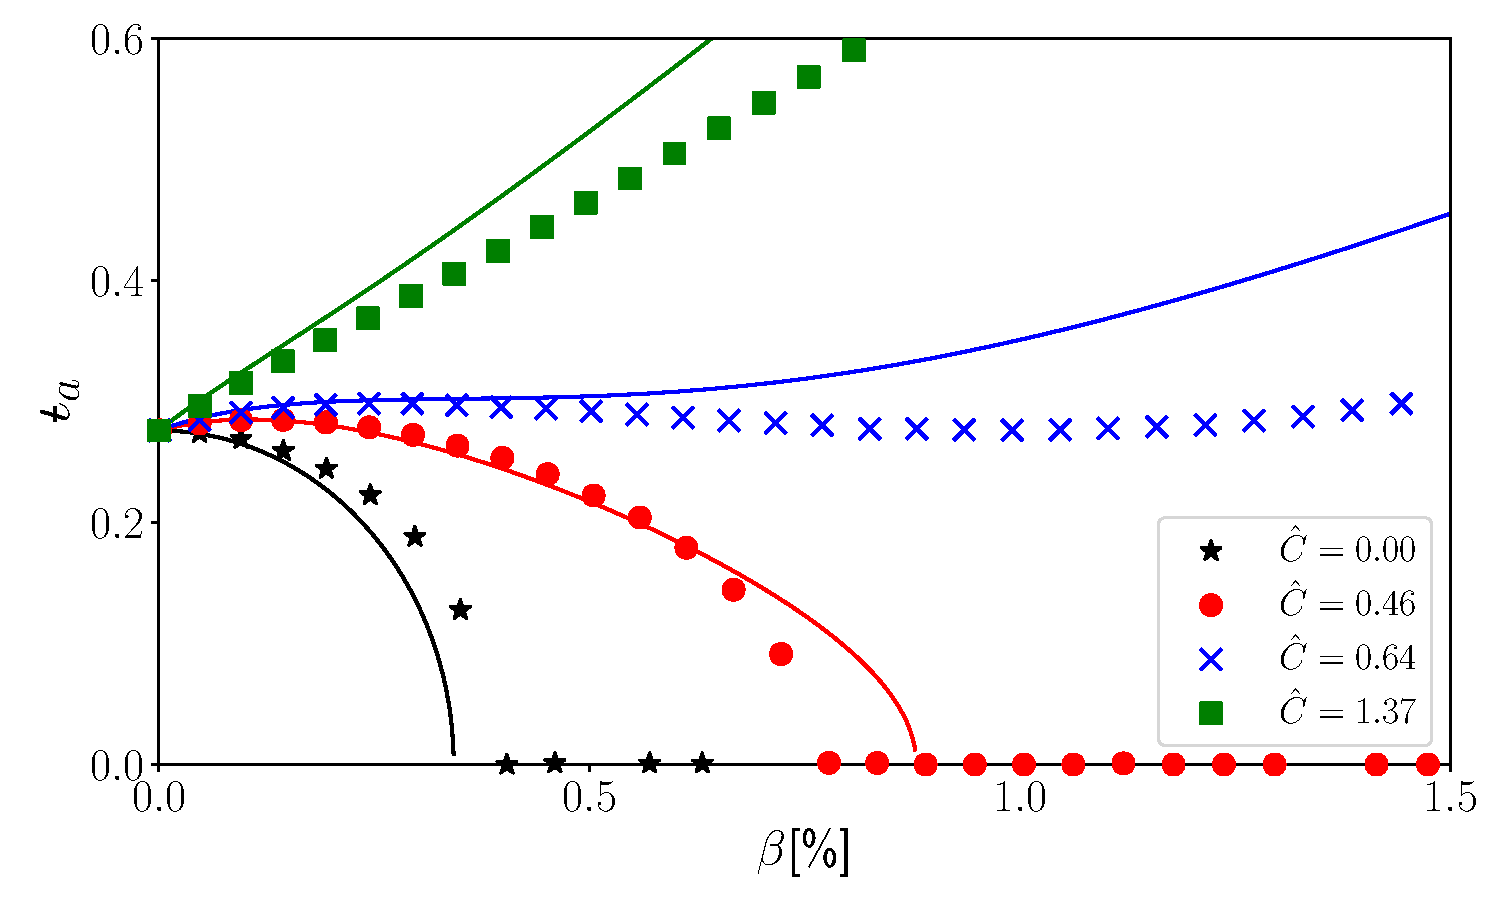
\includegraphics[width=\linewidth]{images/ClassicalStellaratorBetaLimit/iota_edge.pdf}
	\caption{Edge rotational transform, $\iotabar_a$, as a function of plasma average $\beta$, for different values of $\hat{C}$; stars, circles, crosses and squares are SPEC calculations while full lines are given by Eq.(\ref{eq.iota_hbs}).}
	\label{fig. iota edge}
\end{figure}

% Ideal
For small values of $\hat{C}$, namely for $\hat{C} < \hat{C}_{crit}\approx 0.59$, the edge rotational transform decreases with increasing $\beta$ and eventually reaches zero (Figure \ref{fig. iota edge}, black stars and red dots), at which point an $m=1,\ n=0$ island opens and forms a separatrix at the plasma boundary (see left panels of Figure \ref{fig. poincare}). We will refer to this $\beta$-limit as the \emph{ideal equilibrium $\beta$-limit}, denoted by $\beta_{lim}^{ideal}$, since it is well described by ideal MHD theory (see section \ref{sec. ideal limit}). The value of $\beta^{ideal}_{lim}$ obtained with SPEC is shown as a function of $\hat{C}$ in Figure \ref{fig. beta limits} (red triangles).



\begin{figure}
	\centering
	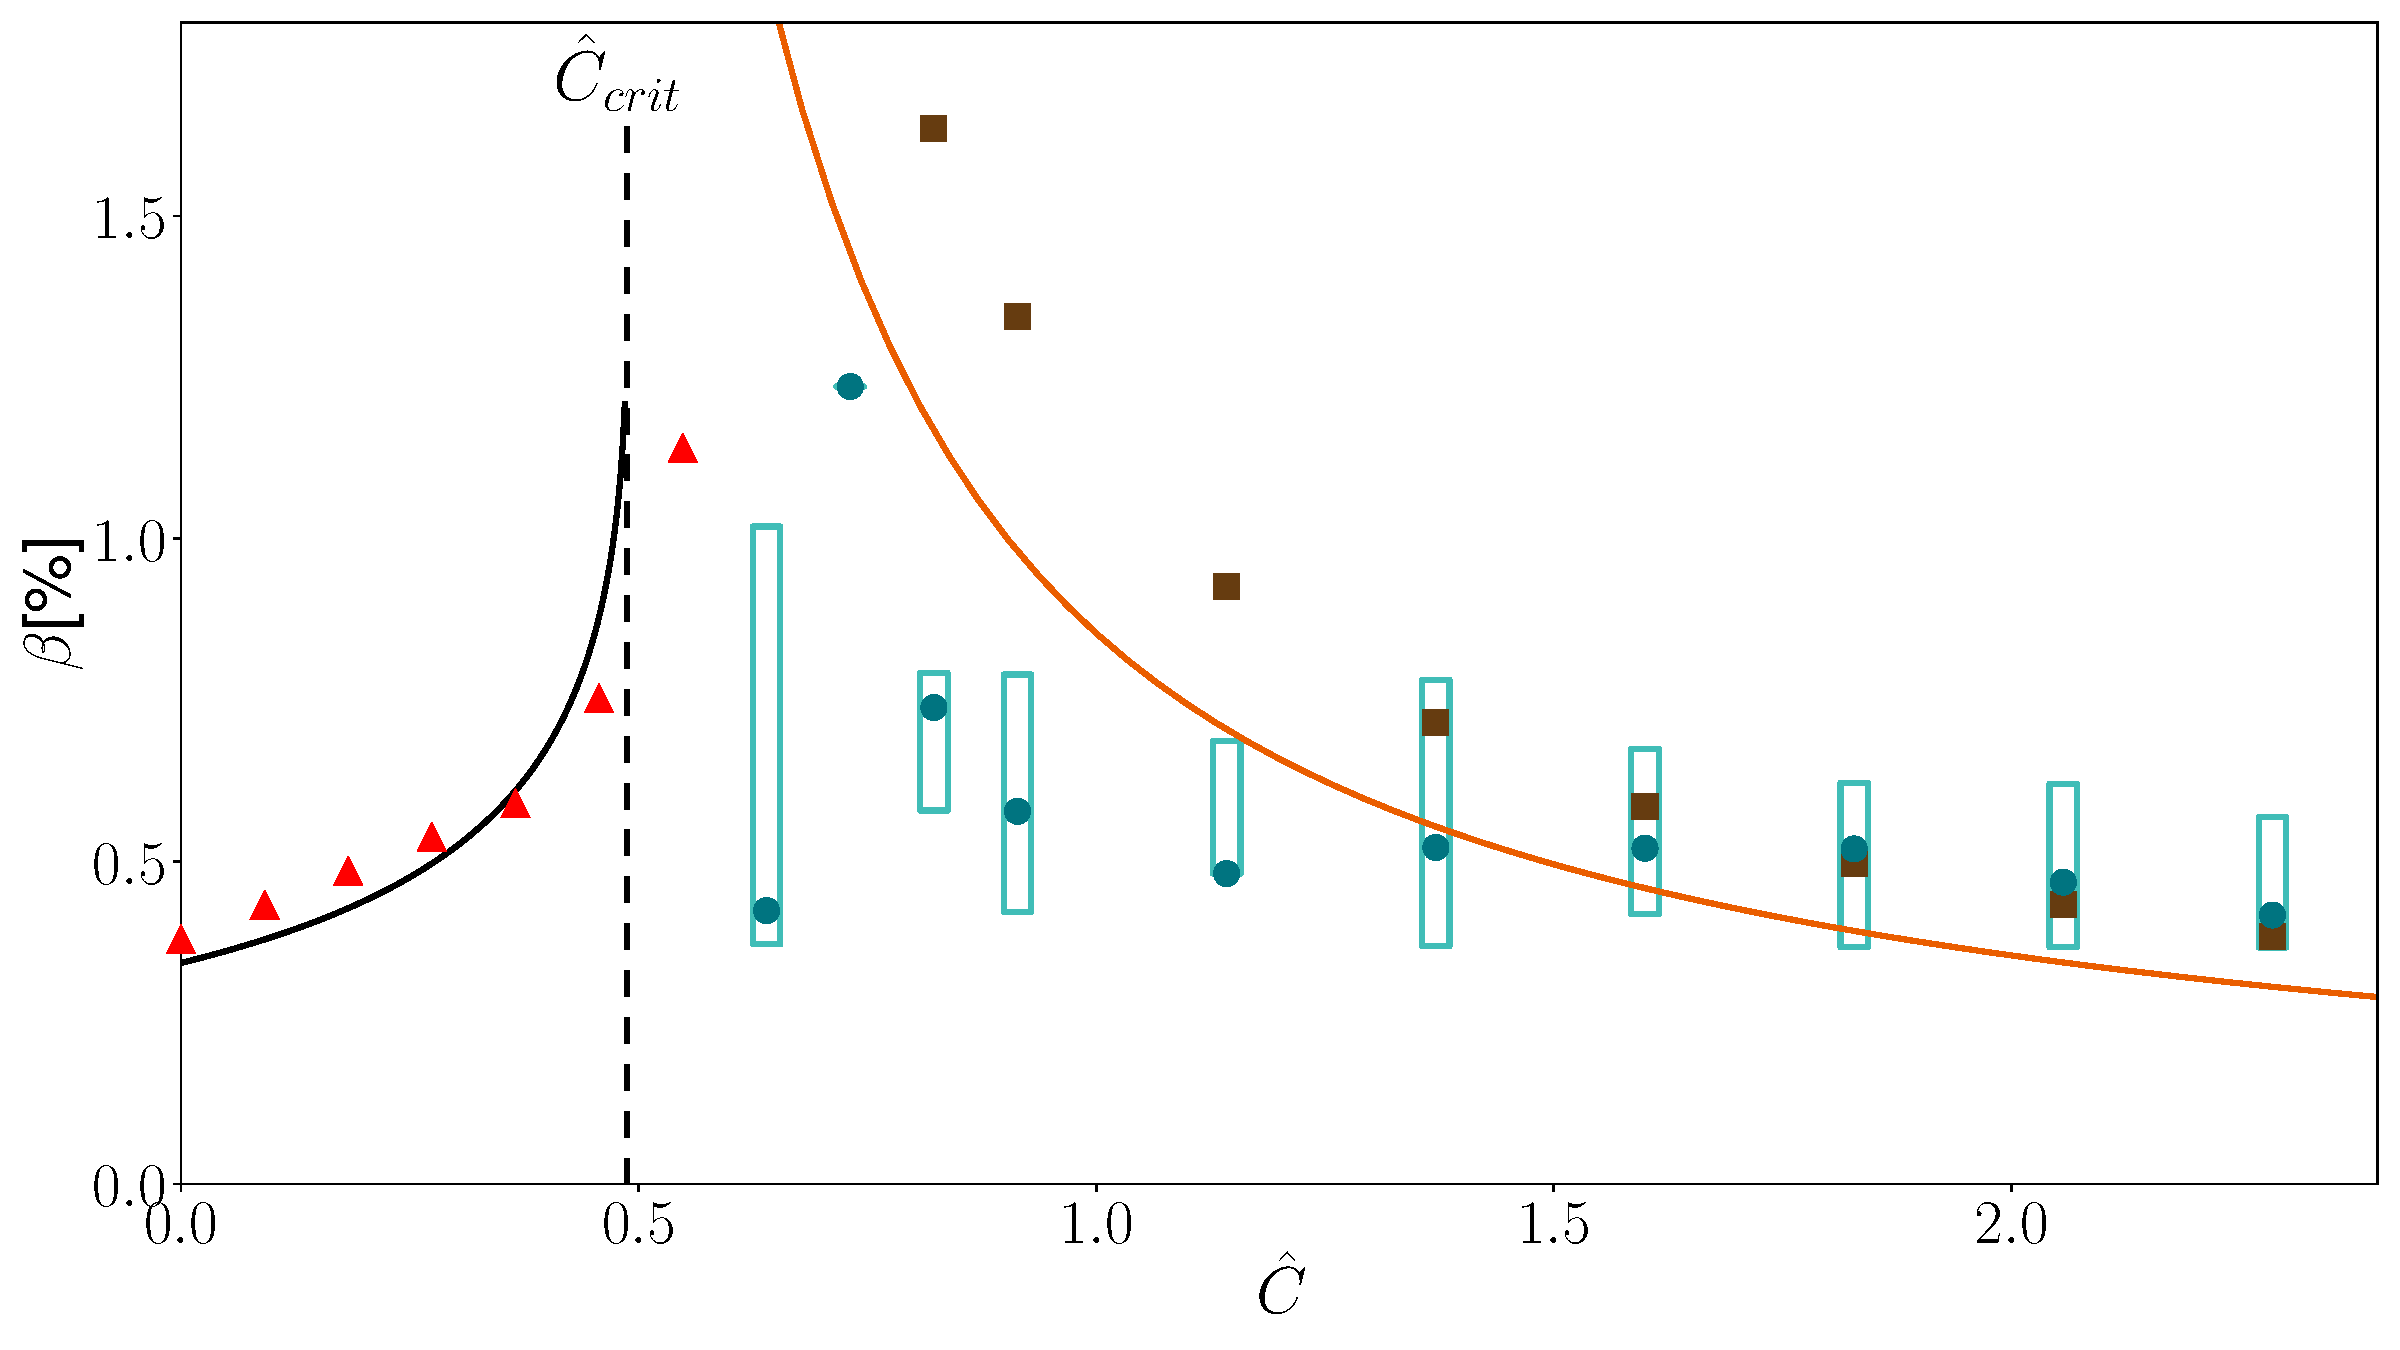
\includegraphics[width=\linewidth]{images/ClassicalStellaratorBetaLimit/beta_limit_dBr=1e-5_NoVacuum.pdf}
	\caption{Equilibrium $\beta$-limit as a function of $\hat{C}$. Red triangles: ideal equilibrium $\beta$-limit, reached when $\iotabar_a=0$, as obtained from SPEC. Black solid line: analytical prediction for $\beta^{lim}_{ideal}$ from Eq.(\ref{eq.hbs ideal limit}). The dashed vertical line indicates the analytical value of $\hat{C}_{crit}$ from Eq.(\ref{eq.Ccrit analytical}). Blue: chaotic equilibrium $\beta$-limit, as obtained from SPEC, with dots indicating the values obtained for $ B_{r,crit}/B=10^{-5}$, and the rectangular boxes showing the range obtained for $ B_{r,crit}/B\in[10^{-6},10^{-4}]$. Orange: analytical prediction obtained by solving from Equation (\ref{eq.hbs chaos limit}) and brown squares: SPEC values for which $\iotabar_a=2\iotabar_v$.}
	\label{fig. beta limits}
\end{figure}


The ideal equilibrium $\beta$-limit can also be observed in tokamaks, although the underlying mechanism is different. In a tokamak, the plasma may be kept centered by applying a vertical magnetic field $B_Z$. As $\beta$ grows, $B_Z$ has to be increased, until it compensates the poloidal field $\mathbf{B}_p$ on the high field side. When this happens, the field is purely toroidal and a separatrix opens.
In a stellarator, the poloidal magnetic field does not have to cancel everywhere for a separatrix to open, it merely has to be such that a field line never completes a poloidal turn. If this happens, the edge rotational transform is zero and a separatrix opens.
In our calculations, the net toroidal current is constrained in the plasma volumes and at the interfaces. However the actual dependencies of the current density on the toroidal and poloidal angle are unconstrained. Pfirsch-Schl\"uter and diamagnetic currents angular dependencies are the source of the poloidal magnetic field perturbation, the lowering of the edge rotational transform, and ultimately the opening of the separatrix. This is why, even in a zero net-toroidal-current stellarator ($\hat{C}=0$), the edge rotational transform reaches zero.

% Chaos
For values of $\hat{C}>\hat{C}_{crit}$, the (now strong enough) bootstrap current is able to prevent the edge rotational transform from reaching zero for any $\beta$, and hence no $m=1,\ n=0$ island appears anywhere (see the blue crosses and green squares in Figure \ref{fig. iota edge}). 
Instead, the edge rotational transform increases until many island chains open in the plasma and in the vacuum region (right panels of Figure \ref{fig. poincare}). When these islands are large enough to have a significant impact on the radial transport, the \emph{chaotic equilibrium $\beta$-limit} is reached, denoted by $\beta_{lim}^{chaos}$. Finally, for all values of $\hat{C}$, islands start to overlap and generate large regions of chaotic field lines at sufficiently large values of $\beta$ (bottom panels of Figure (\ref{fig. poincare})).

It may be argued that volume interfaces might not be able to support the pressure if islands or chaos are close by (see, for example, the bottom right panel in Fig.\ref{fig. poincare}) --- \textit{i.e.} that SPEC equilibria might not be trusted at large $\beta$ without further analyses. This question has been thoroughly studied in slab geometry by \citet{Qu2021}. They identified two reasons why a solution might not exist.

%: either (i) the pressure jump supported by an interface is too large or (ii) the magnetic surface does not exist and is fractal, and cannot be expressed by Fourier series. 

The first possibility is that the magnetic surface does not exist, in particular that it is fractal. In our calculations above the equilibrium $\beta$-limit, large magnetic islands and chaotic regions develop close to volumes interfaces. In this situation, it is indeed not known if the solution exists and additional analyses would be required, for example with convergence studies as proposed by \citet{Qu2021}.  Below the equilibrium $\beta$-limit, however, only small islands are present. The interfaces are not perturbed by neighbouring, large magnetic islands, and it is likely that the volume interfaces are magnetic surfaces. Since we are only interested in computing the equilibrium $\beta$-limit, it is sufficient to calculate equilibria \emph{below or equal to} the equilibrium $\beta$-limit; larger $\beta$ equilibria are irrelevant, and thus the question of existence of interfaces is eluded.

The second possibility is that the pressure jump on an interface is too large and a solution to the force-balance equation (\ref{eq. force balance}) does not exist. This is a possible explanation for when SPEC does not find an interface geometry that satisfies the force balance equation, Eq.(\ref{eq. force balance}). However, in our calculations, SPEC finds magnetic geometries that do satisfy force balance. This means that the pressure jump across the interfaces is small enough and a solution exists. To summarize this discussion, we can trust SPEC solutions for all $\beta$ smaller or around the equilibrium $\beta$-limit, which is sufficient for the study presented in this paper.

To evaluate the chaotic equilibrium limit numerically, the volume of chaos ($V_{chaos}$) introduced in section \ref{sec.volume chaos} can be leveraged. The chaotic equilibrium $\beta$-limit could then be defined as the $\beta$ above which $V_{chaos}>0$. The volume of chaos, however, while very useful as a measure of the amount of chaotic field lines, does not provide enough information about whether or not the radial transport is enhanced by the destruction of magnetic surfaces. In addition, the volume of chaos is sensitive to the numerical resolution of the equilibrium --- the larger the number of Fourier modes, the greater the number of potential resonances in the equilibrium. Due to overlap between small islands chains generated by high order rationals, chaos may emerge at smaller $\beta$ as the Fourier resolution is increased. For example, in Figure \ref{fig. metrics convergence} the volume of chaos is plotted as a function of $\beta$ for two different Fourier resolutions, $M=N=6$ and $M=N=10$ (blue lines). We see that with this diagnostic, the measured chaotic equilibrium $\beta$-limit would drop from $\sim 1.5\%$ to $\sim 1\%$ if it were defined as the $\beta$ above which $V_{chaos}>0$. However, in the $M=N=10$ scan, some of the chaotic field lines are formed by high order rationals and their associated smaller islands are expected to participate weakly to the radial transport, and could potentially be ignored.

\begin{figure}
	\centering
	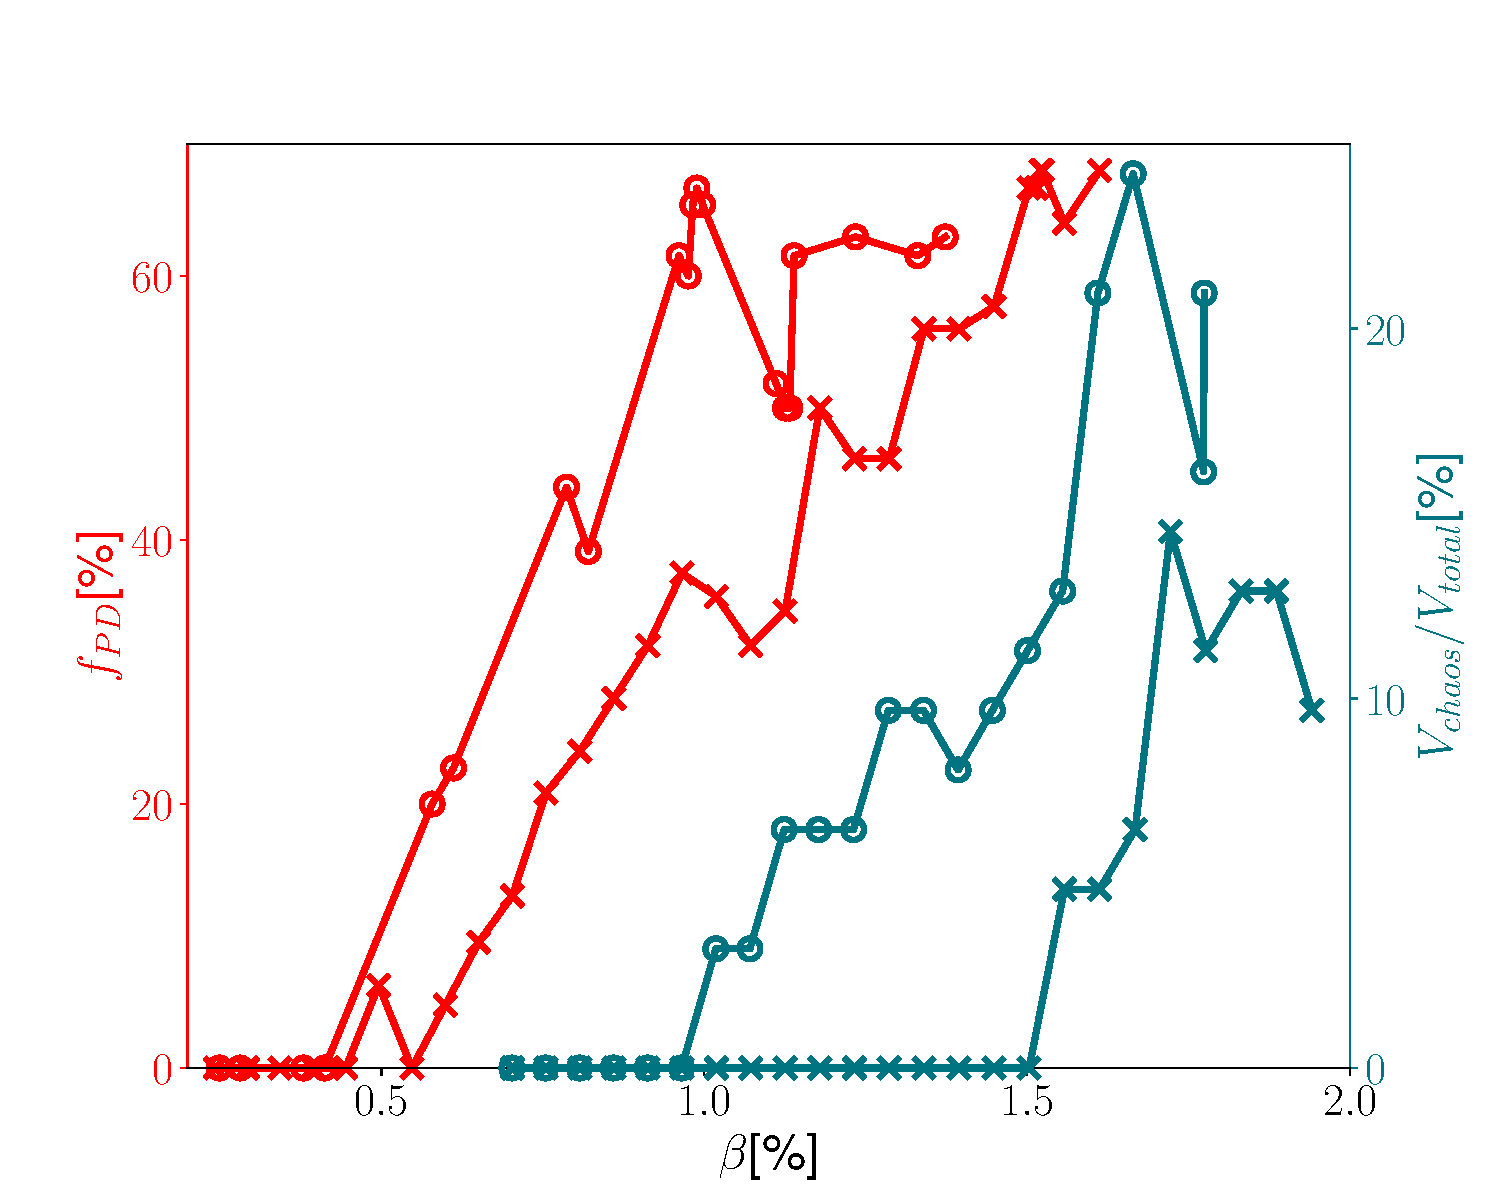
\includegraphics[width=0.75\linewidth]{images/ClassicalStellaratorBetaLimit/dBr_versus_Vchaos_convergence.pdf}
	\caption{$V_{chaos}/V_{total}$ (blue), and $f_{PD}$ evaluated for $ B_{r,crit}/B=10^{-5}$ (red) versus plasma averaged $\beta$, for $M=N=6$ (crosses) and $M=N=10$ (circles).}
	\label{fig. metrics convergence}
\end{figure}

Instead, we define the equilibrium $\beta$ limit as the $\beta$ above which the volume of effective parallel diffusion, $V_{PD}$, is greater than zero (see section \ref{sec.fraction parallel diffusion}). To evaluate this critical $\beta$, we use the fraction of effective parallel diffusion $f_{PD}$ as a proxy function. With this definition, only resonances with large radial magnetic field component matter (we recall that the radial direction is the direction perpendicular to isotherms); increasing the Fourier resolution of the equilibrium only introduces resonances with small radial magnetic field components, and thus does not impact the value of $f_{PD}$ --- see for example the comparison between two $\beta$-scans with resolution $M=N=6$ and $M=N=10$ in Figure \ref{fig. metrics convergence} (red curves). The critical $\beta$ at which $f_{PD}$ becomes larger than zero is quite insensitive to the Fourier resolution. In that sense, this new diagnostic is more robust than the diagnostic based on the volume of chaos.

Note that this does not define an equilibrium $\beta$-limit from an experimental point of view --- the metric $f_{PD}$ is positive as soon as one resonance satisfies Eq.(\ref{eq.bcrit_estimate}), which would, in practice, only flatten the temperature and density profiles locally. It is certainly possible to increase the plasma averaged $\beta$ further by increasing the input power. Our metric $f_{PD}$ however informs us that the effect of field line topology starts to become important and has to be taken into account in transport calculations for $\beta>\beta^{chaos}_{lim}$. One could imagine to combine the volume of chaos given by Eq.(\ref{eq.volume chaos}) with the criterion given by Eq.(\ref{eq.bcrit_estimate}), and only consider resonances that span a sufficiently large volume \emph{and} that contribute significantly to the radial transport. This idea will not be explored in this paper, and is left for future studies.	

The chaotic equilibrium $\beta$-limit obtained using the metric $f_{PD}$ defined in Eq.(\ref{eq.def metric}) is plotted in Figure (\ref{fig. beta limits}) with blue rectangles, spanning the range of $\beta_{lim}^{chaos}$ obtained when varying $ B_{r,crit}/B$ from $10^{-6}$ to $10^{-4}$. The value of $\beta^{chaos}_{lim}$ obtained for $ B_{r,crit}/B = 10^{-5}$ is shown with blue dots. We observe that the largest $\beta$-limit occurs at $\hat{C}\approx0.75$. A small, but non-zero bootstrap current thus \emph{increases} the equilibrium $\beta$-limit with respect to a classical stellarator without any net toroidal current ($\hat{C}=0$), and is thus beneficial. An analytical model that explain the results will be derived in section \ref{sec. chaos limit}.

In practice, the metric $f_{PD}$ is greater than zero when relatively small islands in comparison to the plasma minor radius emerge (using $ B_{r,crit}/B=10^{-5}$). Thus, as long as the SPEC volumes are large enough to allow these islands to grow, the number of volumes does not affect the metric evaluation. In addition, given a sufficiently large number of volumes, the pressure profile is well resolved by the stepped-pressure approximation and thus the equilibrium does not depend strongly on the number of volumes. In summary, the number of volumes has to be large enough to resolve well the pressure profile, but small enough to allow islands to grow --- this is how it has been decided to use seven plasma volumes (and one vacuum region).




\subsection{Analytical prediction for the equilibrium $\beta$-limits}\label{sec.analyticalmodel}

%\item  We use the so-called "overlap equation", obtained by considering the overlap regime between the Greene-Johnson model \citep{Greene1961} and the High Beta Stellarator (HBS) expansion \citep{Freidberg2014, wakataniStellaratorHeliotronDevices1998}. The derivation of the equation requires a substantial amount of algebra, detailed by \citet{Freidberg2014}, and summarized by \citet{Loizu2017}. This model is valid for $\epsilon\ll1$, $\delta=|\mathbf{B}_p|/B_\phi\sim\epsilon^{3/4}$ with $\mathbf{B}_p$ the poloidal magnetic field, $\beta\sim\epsilon$ and $N_{fp}\sim\epsilon^{-1/2}$, all orderings satisfied by our constructed equilibrium.
%\item Assuming a linear pressure profile $dp/d\psi_p=\text{cst}$ and a poloidal averaged toroidal current density $\langle j_\phi\rangle=A+C\langle x \rangle$, with
%\begin{equation}
%	\displaystyle\langle Q \rangle = \frac{\oint Q \frac{dl_p}{|\nabla_\perp\psi_p|}}{\oint \frac{dl_p}{|\nabla_\perp \psi_p|}},
%\end{equation}
%where the integrals are performed along a poloidally closed loop, and $\nabla_\perp = \nabla - (\mathbf{B}/|\mathbf{B}|)\cdot\nabla$, and assuming circular magnetic surfaces, the overlap equation can be solved. Of particular interest is the analytical prediction for the rotational transform at the plasma edge,

We now derive an analytical model that predicts both the ideal and chaotic equilibrium $\beta$-limits. We make use of high-$\beta$ stellarator expansion theories derived by \citet{wakataniStellaratorHeliotronDevices1998,Freidberg2014} to describe how the rotational transform at the plasma edge $\iotabar_a$ evolves with $\beta$, taking into account the effect of the bootstrap current as well. Once a formula for $\iotabar_a(\beta)$ has been derived, we can find whether an ideal $\beta$-limit is reached by solving $\iotabar_a(\beta)=0$. When no solution is possible, a chaotic $\beta$-limit may also be estimated by assuming that the edge iota is modified by order one with respect to the vacuum rotational transform, $\iotabar_a(\beta)-\iotabar_a(0) \sim \iotabar_a(0)$, at which point it is likely that many resonances exist. 

Assuming that (i) $\epsilon\ll1$, $\delta=|\mathbf{B}_p|/B_\phi\sim\epsilon^{3/4}$ with $\mathbf{B}_p$ the poloidal magnetic field, $\beta\sim\epsilon$ and $N_{fp}\sim\epsilon^{-1/2}$, that (ii) magnetic surfaces are circular, and (iii) considering Solove'v profiles for the pressure $dp/d\psi_p=\text{const}$, and the surface averaged toroidal current density $\langle j_\phi\rangle=\text{const}$, one can derive \citep{wakataniStellaratorHeliotronDevices1998,Freidberg2014} an analytical model for the edge rotational transform,
\begin{align}
	\iotabar_a &= (\iotabar_I+\iotabar_v)\sqrt{1-\nu^2}\label{eq.iota_hbs}\\ 
	\text{with}\ \iotabar_I &= 
	\frac{R_0}{2\psi_a}\mu_0I_\phi(\beta)\\ \label{eq.iota i}
	\text{and}\ \nu &= \frac{\beta}{\epsilon_a(\iotabar_I+\iotabar_v)^2},
\end{align}
where $I_\phi$ is the net toroidal current enclosed by the plasma and $\iotabar_v$ is the edge rotational transform in vacuum.

The bootstrap current model we employed in our equilibrium calculations (Eq.(\ref{eq.bootstrapmodel})) implies a linear relation between the net toroidal current in the system and the plasma $\beta$, thus
\begin{equation}
	\iotabar_I = \sigma\beta,
\end{equation}
where $\sigma$ is a proportionality constant. It can be related to $C$ by integrating Eq.(\ref{eq.current density continuous}) to compute $I_\phi$ in Eq.(\ref{eq.iota i}), leading to

\begin{equation}
	\sigma = \frac{2}{5}\frac{1}{\pi \epsilon_a^{3/2}\iotabar_v}\hat{C}.\label{eq.kappa-C}
\end{equation}

Combining Eqs.(\ref{eq.iota_hbs})-(\ref{eq.kappa-C}), analytical expressions of the edge rotational transform as a function of $\beta$ for different values of $\hat{C}$ can be obtained. Figure \ref{fig. iota edge} compares the analytical curves to results obtained with SPEC.  We observe reasonable agreement especially at low $\beta$. As $\beta$ increases however, Eq.(\ref{eq.iota_hbs}) consistently underestimates the actual value of the rotational transform found by SPEC. Thus, even though the equilibrium constructed in section \ref{sec.equil} does not exactly satisfy the assumptions used to derive Eq.(\ref{eq.iota_hbs}), the assumptions are reasonable enough to use this analytical model to understand our numerical results. Equation (\ref{eq.iota_hbs}) provides indeed an analytical (non-linear) relation for $\iotabar_a(\beta)$ which can be used to predict both the ideal and chaotic $\beta$-limits, as described in the following subsections.




\subsubsection{Ideal equilibrium $\beta$-limit \label{sec. ideal limit}}
The solution to the relation $\iotabar_a(\beta^{ideal}_{lim})=0$ is given by
\begin{align}
	\beta^{ideal}_{lim} = \frac{1}{\epsilon_a\sigma^2}\left[\frac{1}{2}-\iotabar_v\epsilon_a\sigma - \sqrt{1-4\iotabar_v\epsilon_a\sigma}\right], \label{eq.hbs ideal limit}
\end{align}
which is real for $\sigma<(4\iotabar_v\epsilon_a)^{-1}$, or 
\begin{equation}
	\hat{C} \leq \frac{5}{8}\frac{\psi_a}{\epsilon_a^{3/2}R_0^2B_0} \equiv \hat{C}_{crit}. \label{eq.Ccrit analytical}
\end{equation}
Note the limit
\begin{equation}
	\lim_{\sigma\rightarrow 0}\beta^{ideal}_{lim} = \epsilon_a\iotabar_v^2, \label{eq. beta limit C=0}
\end{equation}
retrieving the result from \citet{Freidberg2014} and \citet{Loizu2017} for a zero-net-current stellarator ($\hat C=0$).

The curve $\beta^{ideal}_{lim}(\hat{C})$ is plotted in Figure \ref{fig. beta limits} with a black line. We observe that as $\hat{C}$ increases, the ideal equilibrium $\beta$-limit increases. Comparison with data points measured from SPEC equilibria (red triangles) shows good agreement, especially for weaker bootstrap current ($\hat C<0.5$). The analytical value of $\hat{C}_{crit}\approx0.48$ is reasonably close to the one obtained with SPEC (smaller by about $18\%$).

%Again, the general trend of the ideal equilibrium $\beta$-limit has been recovered by the analytical model (\ref{eq.hbs ideal limit})
	


\subsubsection{Chaotic equilibrium $\beta$-limit \label{sec. chaos limit}}
For larger values of $\hat C$, \textit{i.e.} $\hat{C}>\hat{C}_{crit}$, the equilibrium $\beta$-limit is due to the emergence of chaos and its effectiveness in increasing the transport, thus estimating the chaotic equilibrium $\beta$-limit with Eq.(\ref{eq.iota_hbs}) is not trivial - it is not known, \textit{a priori}, which resonance will participate to the radial transport first. However it is reasonable to assume that when the bootstrap current modifies the edge rotational transform by order one with respect to $\iotabar_v$, \textit{i.e.}
\begin{equation}
	\Delta\iotabar_a\equiv\iotabar_a-\iotabar_v=\iotabar_v, \label{eq.condition chaos}
\end{equation}
magnetic islands and chaos are expected to appear. The values of $\beta$ computed with SPEC at which the condition Eq.(\ref{eq.condition chaos}) is satisfied are plotted with brown squares in Figure \ref{fig. beta limits}. We observe good agreement with the chaotic equilibrium $\beta$-limit (blue dots) for $\hat{C}>1$.
	
We can also directly solve equation (\ref{eq.condition chaos}) using equation (\ref{eq.iota_hbs}). We obtain a fourth order polynomial equation for $\beta$,
\begin{equation}
	\beta^4 + 4\frac{\iotabar_v}{\sigma}\beta^3 + \left(2\frac{\iotabar_v^2}{\sigma^2}-\frac{1}{\epsilon_a^2\sigma^4}\right)\beta^2 - 4\frac{\iotabar_v^3}{\sigma^3}\beta - 3\left(\frac{\iotabar_v}{\sigma}\right)^4 = 0. \label{eq.hbs chaos limit}
\end{equation}

The real, positive root of Eq.(\ref{eq.hbs chaos limit}) is plotted with an orange line in Figure \ref{fig. beta limits}. Direct comparison with the numerical data (brown squares) shows that Eq.(\ref{eq.hbs chaos limit}) consistently underestimates the values of $\beta$ that satisfy Eq.(\ref{eq.condition chaos}); this is a direct consequence of the underestimate of $\iotabar_a$ by the analytical model (Figure \ref{fig. iota edge}). The general dependence on $\hat{C}$ is however recovered, capturing the chaotic equilibrium $\beta$-limit trend (blue dots in Figure \ref{fig. beta limits}) observed numerically for values of $\hat{C}>1$. We remark that there are no free parameters in this analytical model. For $\hat{C}_{crit}<\hat{C}<1$, we transition from a low bootstrap current to a large bootstrap current regime. In this region, the edge rotational transform depends weakly on $\beta$ for $\beta\lesssim 1$ (see, for example, the blue crosses in Figure \ref{fig. iota edge}). As a consequence, the solution to Eq.(\ref{eq.condition chaos}) is large, and is therefore a bad estimate for the chaotic equilibrium $\beta$-limit. In this transition region, a more refined model would be required to better reproduce the results.


\subsection{Dependence on design parameters}
The edge rotational transform in vacuum is approximately equal to the rotational transform on axis (low shear configuration), and can be estimated by a zeroth order near axis expansion \citep{helanderTheoryPlasmaConfinement2014,Loizu2017},
\begin{equation}
	\iotabar^{axis}_v\approx\iotabar_v = \frac{N_{fp}}{2}\frac{(r_{max}-r_{min})^2}{r_{max}^2+r_{min}^2}.
\end{equation}


For low values of $\hat{C}$, the ideal equilibrium $\beta$-limit grows with the vacuum rotational transform (see equation (\ref{eq. beta limit C=0})). For example, increasing the number of field periods increases $\iotabar_v$, thus also the equilibrium $\beta$-limit, as shown in Figure \ref{fig. analytical curves}. These results were corroborated by SPEC calculations with $N_{fp}=2$ and $N_{fp}=10$ (data not shown). 


More generally, any mechanism that increases the rotational transform in vacuum will increase the ideal and chaotic equilibrium $\beta$-limits. An increase in rotational transform can be achieved by either increasing the number of field periods, increasing the ellipse eccentricity (\textit{i.e.} increasing the harmonic $R_{11}=Z_{11}$) or adding some torsion to the magnetic axis. Magnetic axis torsion can however have a strong impact on the computed equilibrium, and additional studies would be required to see if it affects the conclusions of this paper.

Equation (\ref{eq.Ccrit analytical}) gives $\hat{C}_{crit}=0.48$, \textit{i.e.} the equilibrium $\beta$-limit is maximized for a bootstrap current that has half the strength of the bootstrap current in an equivalent circular tokamak. Interestingly, if we approximate the total toroidal flux in the plasma as $\psi_a\approx\pi a^2 B_0$, we get $\hat{C}_{crit}=5\sqrt{\epsilon_a}/8$, which only depends on the inverse aspect ratio. 


\begin{figure}
	\centering
	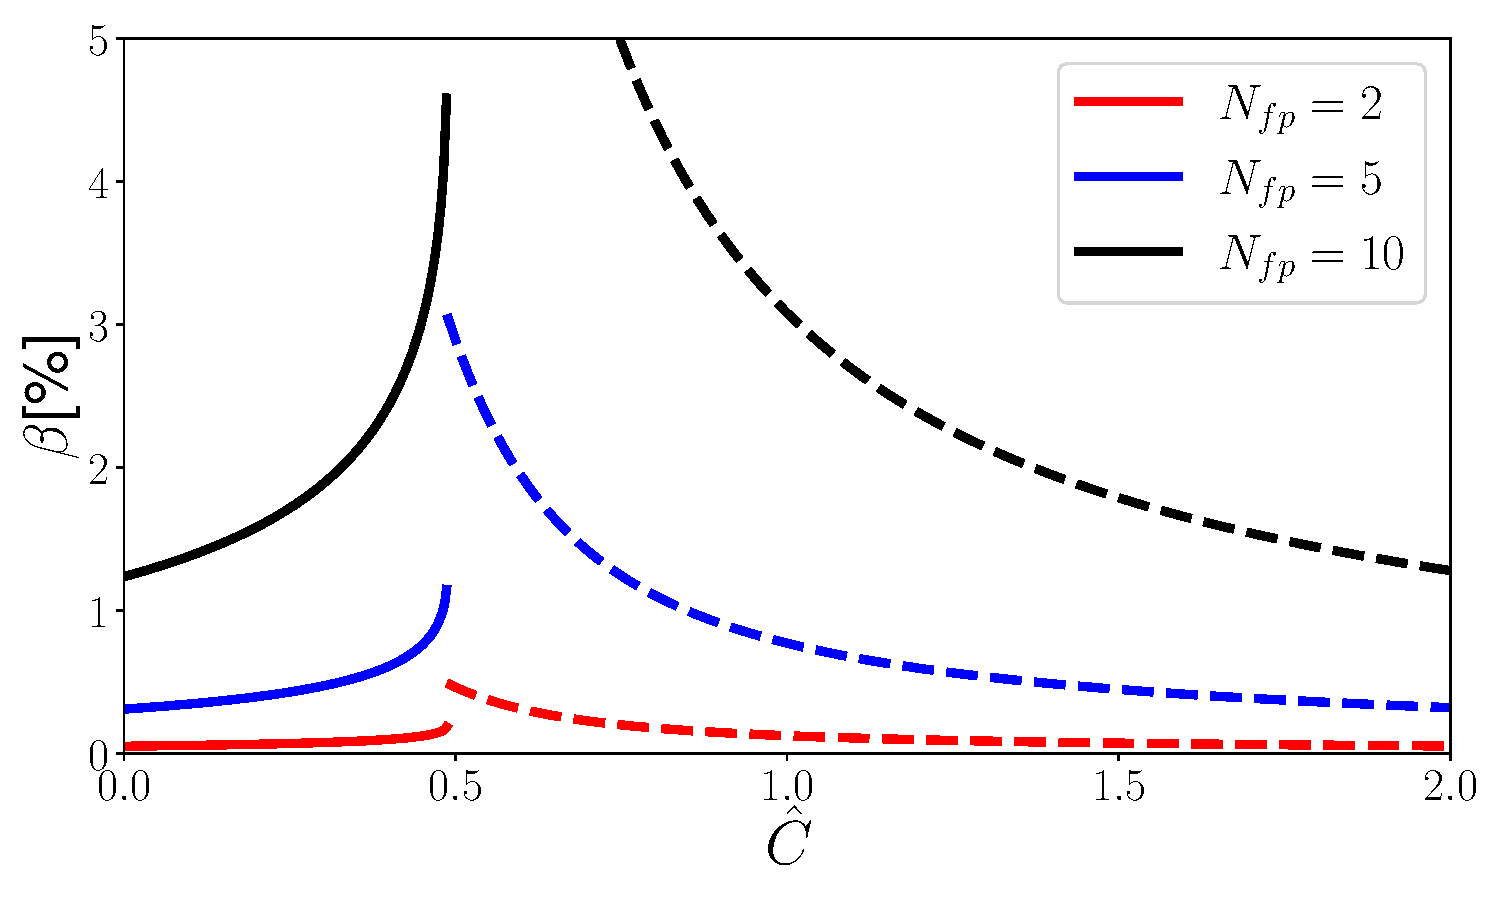
\includegraphics[width=\linewidth]{images/ClassicalStellaratorBetaLimit/beta_limit_analytical_curves.pdf}
	\caption{Analytical predictions of the equilibrium $\beta$-limit for different numbers of field period $N_{fp}$. Full lines: ideal limit ($\iotabar_a=0$) as predicted by Eq.(\ref{eq.hbs ideal limit}), dashed lines: chaos limit ($\iotabar_a=2\iotabar_v$) as predicted by Eq.(\ref{eq.hbs chaos limit})}
	\label{fig. analytical curves}
\end{figure}



% \subsection{Ideal equilibrium beta limit in a classical stellarator} \label{sec.idealbetalimit}

% In this section, it is shown that the \ac{SPEC} current constraint can be used to recover the \ac{HBS} theory prediction of the classical stellarator ideal equilibrium $\beta$-limit \citep{Freidberg2014,wakataniStellaratorHeliotronDevices1998}, when zero net toroidal current is considered.  

% A previous study \citep{Loizu2017} showed remarkable agreement between \ac{SPEC} calculations and the \ac{HBS} theory in a simplified case, with the pressure profile approximated by a single step. An additional limitation, enforced by the \ac{SPEC} version at that time, was that the vacuum region had to be approximated by a large plasma volume where the pressure and currents were set to zero, and a fixed-boundary would be applied. This approach is equivalent to assuming a free-boundary calculation with an infinitely conducting wall at the computational boundary. At large $\beta$, however, a strong Shafranov shift is present, and this approximation could have an impact on the result.

% To understand the effect of these assumptions we consider here both fixed- and free-boundary calculations with a stepped-pressure profile approximating a Solov'ev's profile $p = p_0(1-\psi_t / \psi_a)$ where $\psi_a$ is the total toroidal flux enclosed by the plasma. The computational boundary is defined by Eqs.(\ref{eq.RotEllipse_R})-(\ref{eq.RotEllipse_Z}). Fixed-boundary calculations were made first, with seven plasma volumes surrounded by an eighth large, vacuum-like volume so that it is similar to a free-boundary calculation. The toroidal flux profile has been chosen such that $\psi_a=\sum_{l=1}^7\psi_{t,l}=0.25\text{Tm}^2$ and $\psi_{t,8} = 0.75\text{Tm}^2$, leading to a total toroidal flux enclosed by the plasma and the vacuum-like region of $\sum_{l=1}^8\psi_{t,l} = 1\text{Tm}^2$. Free-boundary input files were generated to replicate the same equilibrium in vacuum, using $\mu_0I_{coil}=21.43$Tm and $\psi_a=0.25\text{Tm}^2$, which correspond to an equilibrium with $\psi_{t,V}=0.75\text{Tm}^2$. In both fixed- and free-boundary calculations, both the surface currents and the volume currents were set to zero, \textit{i.e.} $I_{\phi,l}^{vol} = I_{\phi,l}^{surf} = 0$ for all $l$. The only control parameter remaining is $p_0$, which was increased in order to increase the plasma average $\beta$ until a central $m=1,\ n=0$ island opens. The island emerges when the rotational transform at the plasma edge, $\iotabar_a$, \textit{i.e.} the rotational transform on the outer side of the plasma-vacuum interface, reaches zero (see Figure \ref{fig:poincare}). This is defined as the ideal equilibrium $\beta$-limit. 

% The physical mechanisms leading to the emergence of a separatrix are complex. In brief, the combination of non-zero poloidal harmonics of the Pfirsch-Schlüter and diamagnetic currents at the volumes' interfaces and the effect of the Shafranov shift perturbs sufficiently the poloidal magnetic field so that the rotational transform at the plasma edge decreases, until eventually it reaches zero. These results will be explained in more detail in a future publication.


% The \ac{HBS} theory, building on the pioneering work of Greene and Johnson's stellarator expansion theory \citep{greeneDeterminationHydromagneticEquilibria1961}, predicts that

% \begin{equation}
% 	\iotabar_a = (\iotabar_v + \iotabar_I)(1-\nu^2)^{1/2},\label{eq.HBS_1}
% \end{equation}
% with $\iotabar_v$ the rotational transform at the plasma edge in vacuum and $\iotabar_I$ a contribution from the plasma toroidal current,

% \begin{equation}
% 	\iotabar_I = \frac{\mu_0I_\phi R_{00}}{2\pi a^2B_0},
% \end{equation}
% with $I_\phi$ the total toroidal plasma current, $B_0$ the magnetic field strength on axis and $a$ the effective minor radius at the plasma edge, \textit{i.e.} $a=\sqrt{\psi_a / (\psi_a + \psi_{t,V})} r_{eff}$, with $r_{eff}$ the effective radius of the ellipse, given by the square root of the product between the ellipse major radius $r_{max}=|R_{10}+R_{11}|$ and the ellipse minor radius $r_{min}=|Z_{10}+Z_{11}|$, \textit{i.e.} $r_{eff}=\sqrt{r_{max}r_{min}}$. The parameter $\nu$ is defined as

% \begin{equation}
% 	\nu = \frac{\langle\beta\rangle}{\epsilon_a(\iotabar_v+\iotabar_I)^2},
% \end{equation}
% with $\langle\beta\rangle$ the volume averaged plasma $\beta$ and $\epsilon_a = a / R_{00}$. Setting $\iotabar_a=0$ in Eq.(\ref{eq.HBS_1}) and solving for $\langle\beta\rangle$ leads to a prediction for the ideal equilibrium $\beta$-limit,

% \begin{equation}
% 	\langle\beta\rangle_{lim,HBS} = \epsilon_a(\iotabar_v+\iotabar_I)^2.
% \end{equation}
% In the case of interest, $R_{00}=10$m, $R_{10}=-Z_{10}=1$m, $R_{11}=Z_{11}=0.25$m, leading to $r_{eff}\approx0.97$m and $a\approx0.48$m. Using $I_\phi=0$A, and $\iotabar_v\approx0.28$, one obtains $\langle\beta\rangle_{lim,HBS}\approx0.38\%$.

% \begin{figure}
% 	\centering
% 	\hfill
% 	\subfloat[][$\langle\beta\rangle = 0\%$, $\iotabar_a\approx0.28$]{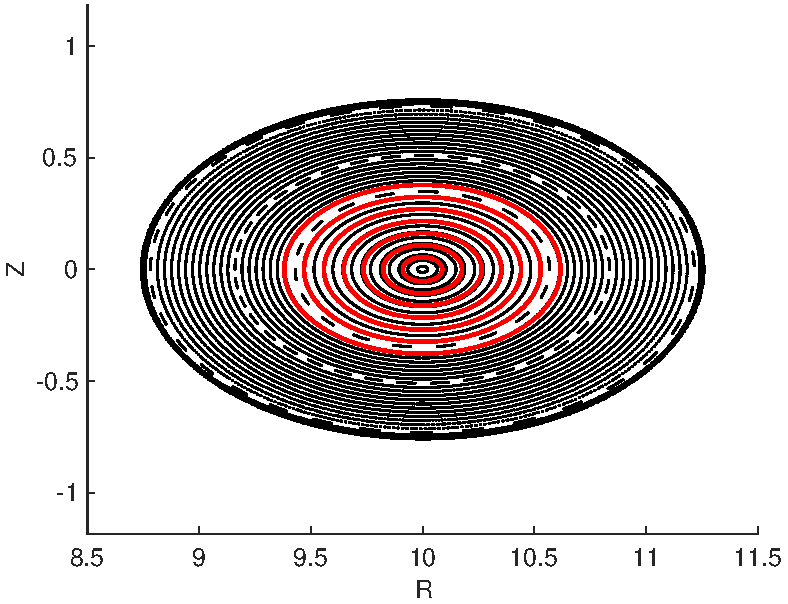
\includegraphics[width=0.3\linewidth]{main/Figures_CurrentConstraint/ABaillod_fig11a.pdf}}
% 	\hfill
% 	\subfloat[][$\langle\beta\rangle \approx 0.31\%$, $\iotabar_a\approx0.13$]{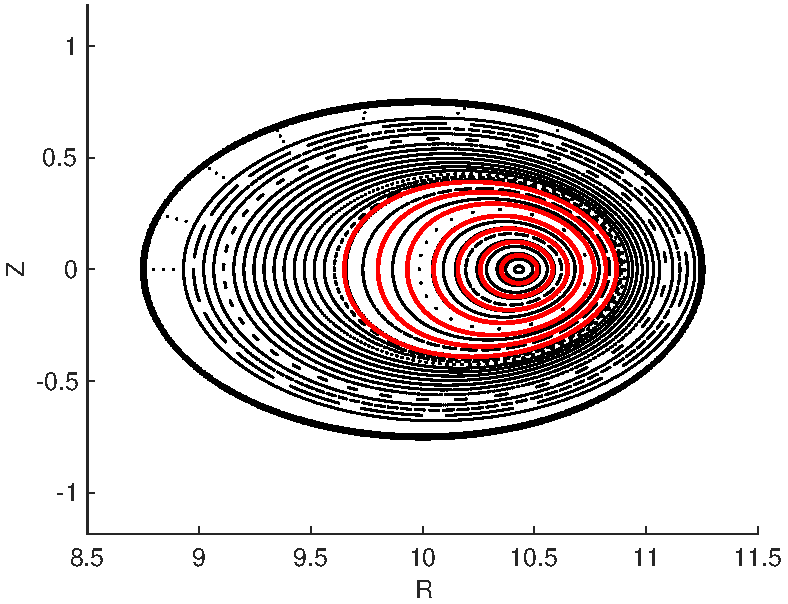
\includegraphics[width=0.3\linewidth]{main/Figures_CurrentConstraint/ABaillod_fig11b.pdf}}
% 	\hfill
% 	\subfloat[][$\langle\beta\rangle \approx 0.62\%$, $\iotabar_a= 0.0$]{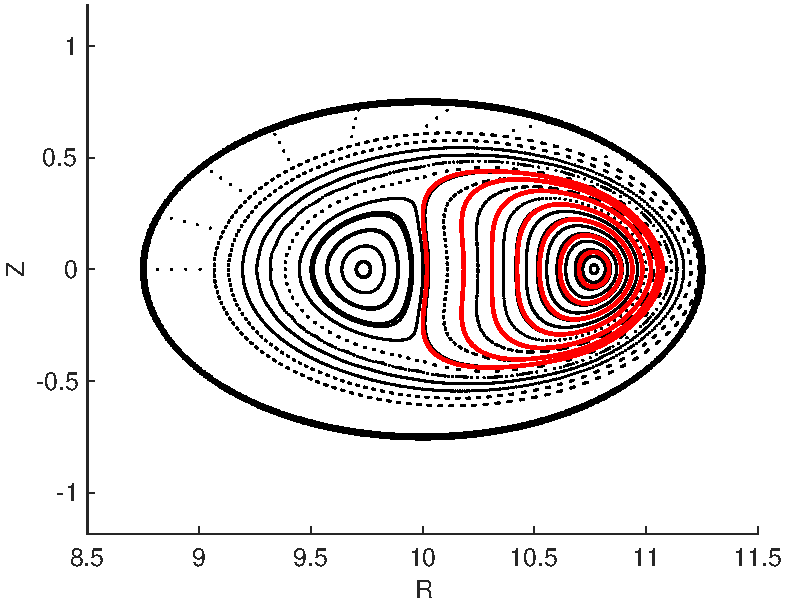
\includegraphics[width=0.3\linewidth]{main/Figures_CurrentConstraint/ABaillod_fig11c.pdf}}
% 	\hfill
% 	\caption{Poincar\'e plot of the magnetic field lines at $\phi=0$ and at three different values of $\langle\beta\rangle$ (a-c). Red surfaces are the volume interfaces and the black, bold surface is the computational boundary. In (c), the ideal equilibrium $\beta$-limit has been exceeded and a central island opened outside the plasma. A large value of $\langle\beta\rangle$ has been selected for illustration purposes.}
% 	\label{fig:poincare}
% \end{figure}

% Figure \ref{fig:iota_beta_scan} shows the rotational transform profile at different values of $\langle\beta\rangle$ (left) and the values of $\iotabar_a$ obtained with \ac{SPEC} as a function of $\langle\beta\rangle$ and compares them to the analytical prediction given by Eq.(\ref{eq.HBS_1}) (right). Good agreement is observed between the fixed-boundary and free-boundary calculations, showing that the fixed-boundary assumption made by \citet{Loizu2017} has only a small effect on the ideal equilibrium $\beta$-limit prediction. In addition, the free-boundary calculation and the \ac{HBS} theory agree well, and predict approximately the same ideal equilibrium $\beta$-limit. The small but finite difference between the results is most likely due to the \ac{HBS} theory, which employs an expansion in aspect ratio $\epsilon$ and assumes that the plasma boundary is circular. In fact, the number of volumes used in \ac{SPEC} to approximate the continuous pressure profile does not significantly influence the result of this study (data not shown).

% \begin{figure}
% 	\centering
% 	\hfill
% 	\subfloat[][]{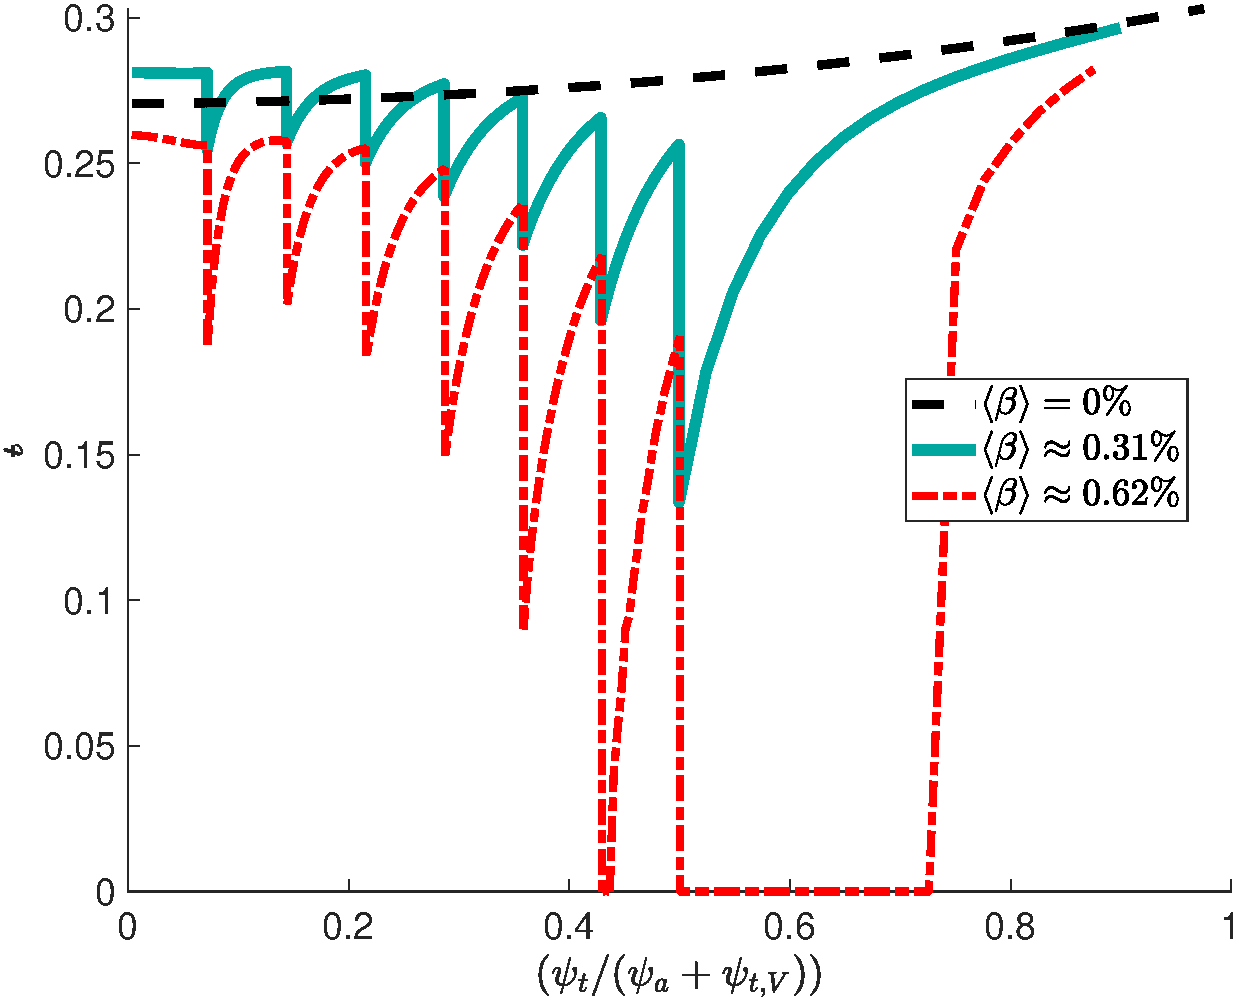
\includegraphics[width=0.45\textwidth]{main/Figures_CurrentConstraint/ABaillod_fig12a.pdf}}
% 	\hfill
% 	\subfloat[][]{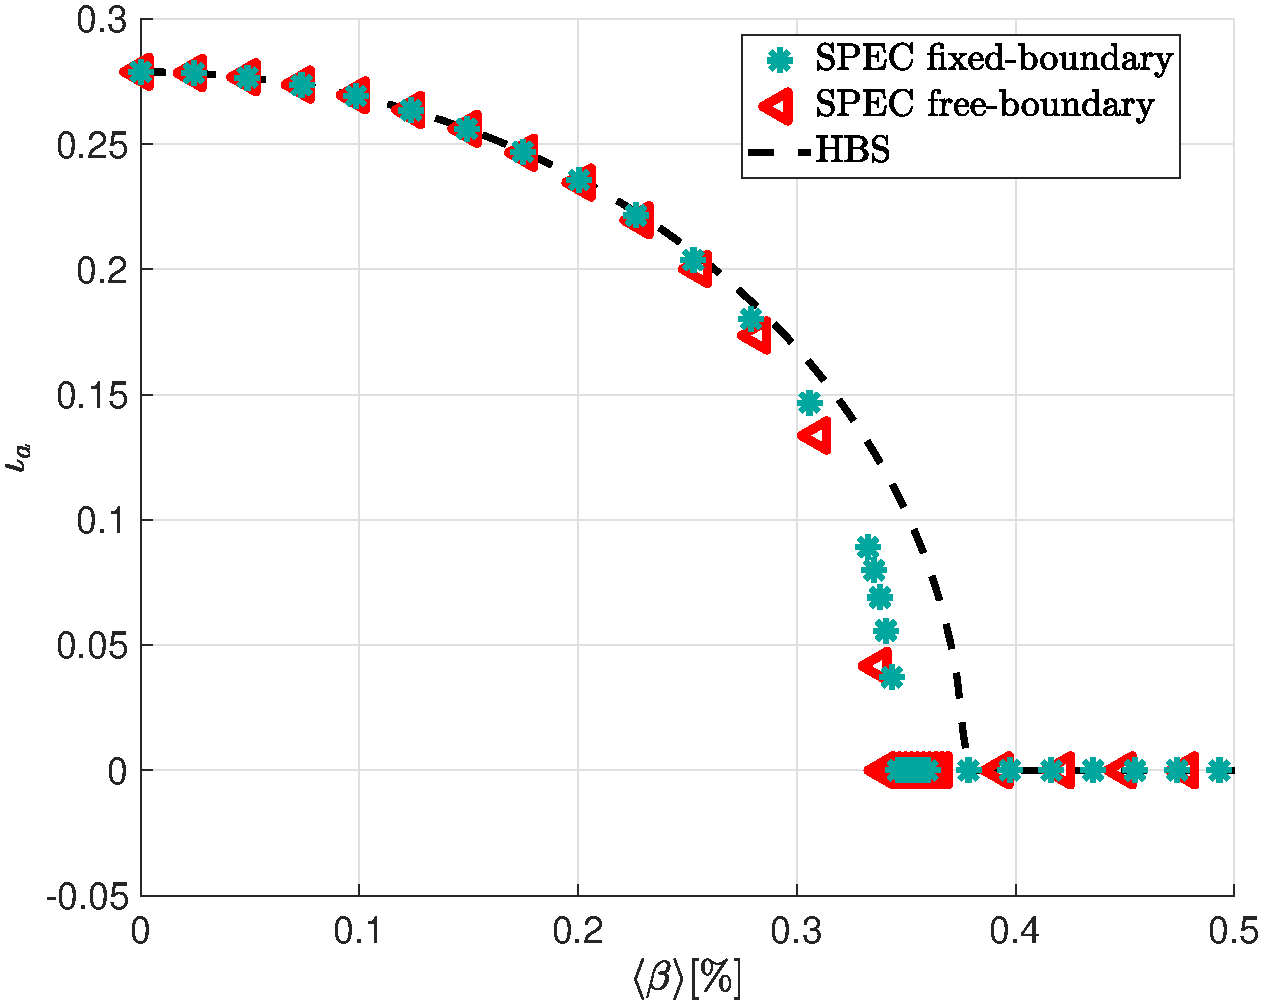
\includegraphics[width=0.45\textwidth]{main/Figures_CurrentConstraint/ABaillod_fig12b.pdf}}
% 	\hfill
% 	\caption{Left: rotational transform profile at three different values of $\langle\beta\rangle$, for free-boundary calculation of a rotating ellipse with zero net toroidal current. Right: rotational transform at the plasma edge as a function of $\langle\beta\rangle$. Comparison between free-, fixed-boundary and the \ac{HBS} theory.}
% 	\label{fig:iota_beta_scan}
% \end{figure}


% As a final remark, note that in our calculations, the plasma boundary is topologically constrained to be an ideal surface and cannot undergo re-connection. Another important constraint is that the pressure profile is fixed and cannot evolve. Other approaches without these constraints could lead to different results and conclusions. One natural question is then to ask about the physical validity of constraining the topology of a set of flux surfaces in \ac{MRxMHD}. First studies about the existence of \ac{MRxMHD} interfaces have been carried out \citep{McGann2010,Qu2021}, pointing towards certain existence criteria. The present study, however, aims at verifying the implementation of the toroidal current constraint in \ac{SPEC} by retrieving well established mathematical results. Future work will focus on code validation by using experimental data.



\section{QA}

\section{QH}

\section{QI}

\end{document}